\chapter{Implementation Environment}
\label{chapter:implenv}
In this chapter, we introduce the environment used for the implementation of this work. Hereby, we provide conceptional overview about the underlying real time critical base implementation, namely ROS\_control, which serves as a generic interface between robot control and respective hardware. At this point, we assume the reader to be familiar with ROS. A good introduction, tutorials and detailed information can be found in \cite{martinez2013learning} and the official website\footnote{\url{http://www.ros.org/}}.

Furthermore, we introduce the SoT as a framework in terms of implementing tasks and dynamically push and pop them on runtime. Hereby, we describe the Dynamic Graph (DG). This serves as a computational graph and each task can be seen as one entity inside this graph.

Latest, the closest points are calculated utilizing an open-source library called Fast Collision Library (FCL), which brings already mechanisms for calculating proximities. During this work, the capabilities of this library is extended for capsules. 

\section{ROS\_control}\label{sec:roscontrol}
In a wide sense, ROS\_control describes a combination of packages for building robot agnostic controllers. It provides interfaces for controllers and various hardware systems to generically separate the controllers from the underlying hardware. ROS\_control thus can be seen as a hardware abstraction layer (HAL). On the upper side, ROS\_control enables a generic ROS compatible programming interface, which allows hardware agnostic computation of various application algorithms. On the lower side, it communicates in a real time safe environment with the concrete hardware. This mechanism is monitored by a independent observer, called the controller manager, which allows to load, switch and unload multiple controllers on runtime. More information can be found in \cite{roscontrol}.

During the development of this work, we implemented a so-called SoT-Controller and integrated it into ROS\_control. This integration implies a seamless migration and execution on the real robot hardware through the implemented HAL for REEMs hardware.
To overcome any real time constraints inside the computation of the stack, we exposed this computation into a separate thread. This not just detaches the SoT from any hard timing condition, but rather allows us to modify the update frequency inside the SoT independently from ROS\_control. At each \texttt{update} function call of the SoT-Controller, it fetches the latest result $q$, representing the accumulated joint states. Those joint state values are passed through a \texttt{joint position controller} and finally to the robots motor controllers. This abstract description is illustrated in figure \ref{fig:sotcontrol}.
\begin{figure}[h!]
  \centering
    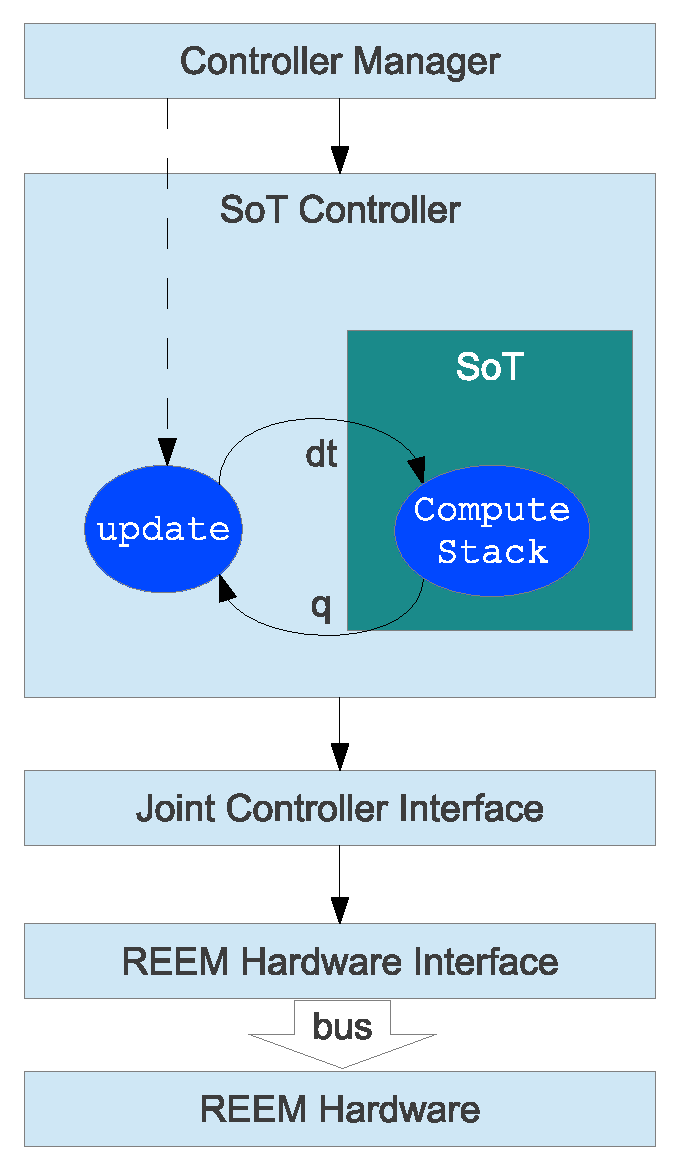
\includegraphics[width=0.4\textwidth]{../figures/sot_controller.eps}
    \caption{Abstract overview of the SoT-controller architecture inside ROS\_control. The controller manager cyclically calls the \texttt{update} function for all subscribed controllers. This update function fetches the latest result from the independently running SoT. The joint states are getting passed over various interfaces finally to the communication bus and the respective motor control boards.}
    \label{fig:sotcontrol}
\end{figure}

\section{Stack of Task - Framework}\label{sec:sotframework}
During the theoretical part in chapter \ref{chapter:soth}, we introduce the SoT as a GIK solver and provide mathematical formulations on how to define a task inside this solver. In this section, we consider the SoT from a software framework point of view. With this being said, in the remainder of this section, the use of the abbreviation SoT refers to the framework rather than the hierarchical solver. 

The SoT comprises mainly two key functionalities. 
\begin{itemize}
\item Dynamic computational graph connecting entities through input/output signals
\item Hierarchical task solver (called sot-core) realized as entities inside the dynamic graph
\end{itemize}

\subsection{Dynamic Graph}
The dynamic graph (DG) provides a computational graph, where entities are connected through input and output signals \cite{mansard:icar:09}. Hereby, every output signal is combined with an internal function of the entity, gathering all necessary information. This happens by consuming the input signals and produce the result on the output signal. Output signals from one entity can be plugged as an input signal of any other entity. 

For every cycle of the control update loop, the DG gets recomputed based on backtracking all linked entities. Triggering an output signal executes the assigned output function inside the entity. Equally, this function might consume linked input signals. Since these input signals represent output signals of other entities, those entities are computed as well. Let us consider the DG illustrated in figure \ref{fig:dg}. In order to calculate the output value of Entity E, all precedent entities are backtracked until the initial values $c_1$ and $c_2$. 

Depending on the size of the DG, this might result in a big overhead of recomputation, even though some entities do not provide new values. In the shown graph, we plug two constant values $c_1$ and $c_2$. Computing now the value of \verb|Entity E| would backtrack the complete graph with no new result, as the initial values are constant. In order to prevent this overhead and recalculate only outdated entities, all signals are time dependent. This timestamp allows a recomputation of the entity only if the according input signals are outdated. 
\begin{figure}[h!]
  \centering
    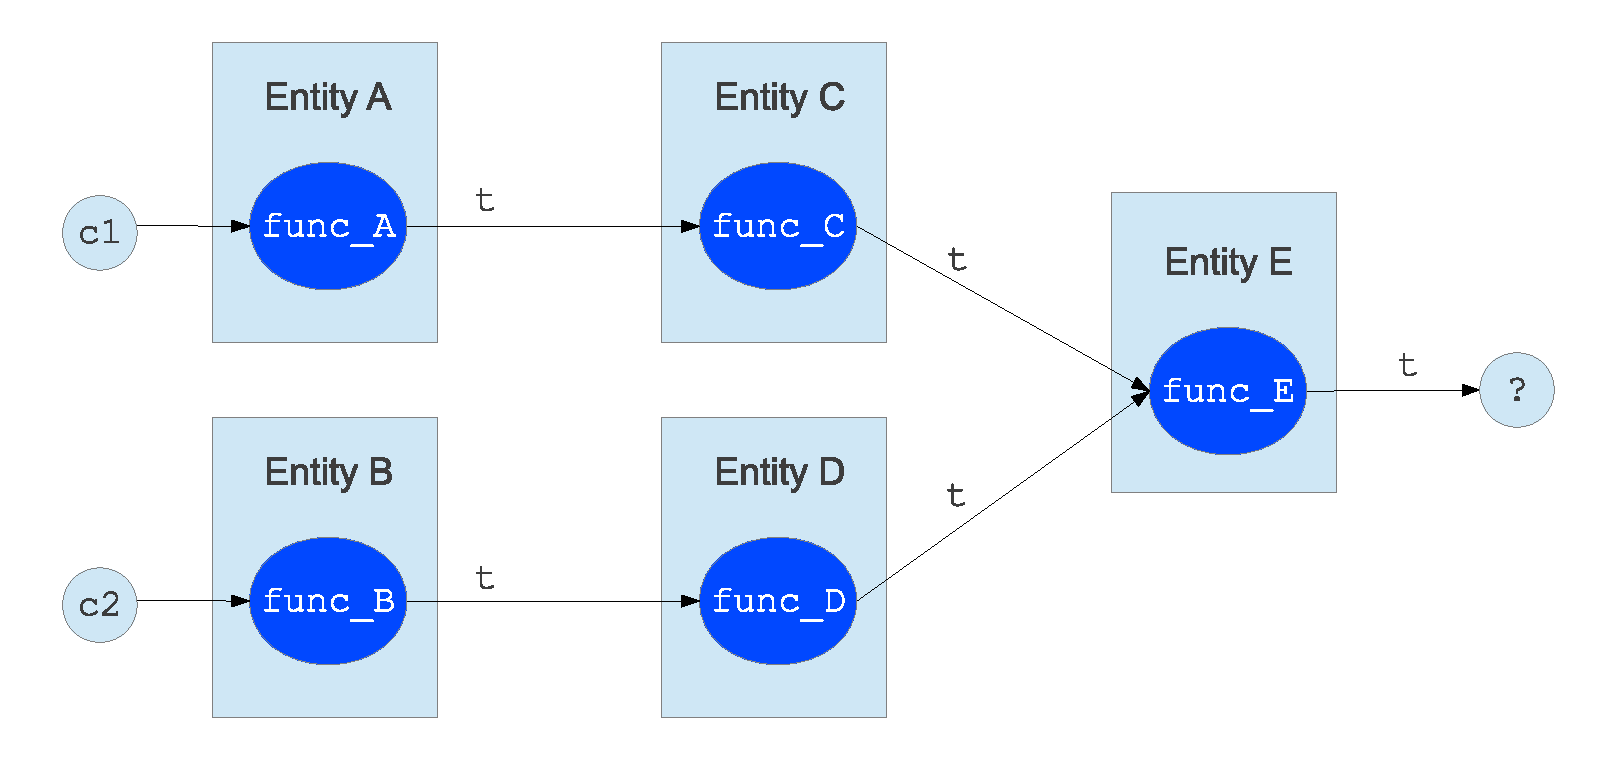
\includegraphics[width=0.8\textwidth]{../figures/dg.eps}
    \caption{Dynamic Graph with five entities $A-E$. Calculating the output of \texttt{Entity E} triggers a recursive backtracking until all entities are updated. In order to prevent an unnecessary recalculation of unchanged entities, signals are computed with a timestamp $t$. This timestamp keeps track of changes, which indicates whether an entity is outdated and has to be recomputed.}
    \label{fig:dg}
\end{figure}
\newpage
An example would be an entity called \textit{feature}, which calculates the error between the actual and desired position of the end-effector position. Thus, this entity comprises two input signals $p(t)$ and $p_{des}(t)$. The respective output signal provides the error, hence the name $e(t)$. The function linked to the output signal obviously computes the difference between $p$ and $p_{des}$ at time $t_i$. Algorithm \ref{algo:feature} describes this simple function, where the two input signals are fetched at the same timestamp and the resulting error is computed. The output signal equals the return value of the function.

\begin{algorithm}[]
\SetAlgoLined
\SetKwInOut{Input}{input}
\SetKwInOut{Output}{output}
\SetKwFunction{getp}{p\_signal\_in}
\SetKwFunction{getpdes}{p\_des\_signal\_in}
/* signals have to be initialized before */ \\
\Input{Timestamp $t$}
\Output{Error $e$}
p = \getp{$t$} \;
p\_des = \getpdes{$t$} \;
e = p\_des - p \;
return e \;
\caption{error computation in entity feature}
\label{algo:feature}
\end{algorithm}

\newpage
\subsection{SoT Core}
As mentioned in the beginning of this chapter, the SoT (meaning the hierarchical solver in this case) is realized as an dedicated entity inside the DG. This entity provides functionalities to dynamically push and pop task entities. 

We described already in the theoretical part, how a task definition looks like. Since we minimize a QP in the form of 
\begin{eqnarray}
\vec{Ax -b} &\quad& \textit{generic form} \notag \\
\vec{J \dot{q} - \dot{e}} &\quad& \textit{inverse kinematic} \notag
\end{eqnarray}
We have to specify the Jacobian $\vec{J}$ as well as the residual $\dot{e}$, which represents \mbox{- in this case -} the error between actual and desired position. 
The interface for a task implementation thus provides two output signals for the Jacobian and the error, respectively. 

In the previous section, we explained how output signals are handled inside the dynamic graph. The assigned output function for each signal is task dependent. An example positioning task for an end-effector can then easily be formulated by using the error calculation of the feature entity (see algorithm \ref{algo:feature}) and the Jacobian for the end-effector. 

We have to point out that at this point, we have only designed a task. We are not solving this task though. The task becomes part of the solver by explicitly pushing it onto the stack. The hierarchical solver in itself describes another entity, which holds all tasks, currently pushed on the stack. This entity solves the stack by fetching all \texttt{jacobian} and \texttt{error} output signals from all tasks. This will be transformed into one big, hierarchy respecting Jacobian and error. This will be finally solved and the result is provided as an output signal. We are not going any deeper into details here. The main information should be the requirements for designing tasks and push them on the stack for getting considered by the solver. Mathematical details can be found in \cite{escande-icra-10}\cite{escande:ijrr:2014}. An deeper insight into the development of the framework is provided in \cite{mansard-tro-09}.

Furthermore, we want to remind that the mathematical solver indeed solves the generic form of the above stated formulations. This being said, there is no need to specify $\vec{A}$ exclusively as a Jacobian matrix. This allows us also to specify tasks directly in joint space. 
\begin{eqnarray}
\vec{Ax -b} &\quad& \textit{generic form} \notag \\
\vec{I \dot{q} - \dot{q}_d} &\quad& \textit{joint space task} \notag
\end{eqnarray}
Where $\vec{I}$ denotes an identity matrix. The residual therefore has to be given in joint space, hence the naming $\vec{q_d}$, which specifies a desired joint velocity.

\section{Fast Collision Library (FCL)}
FCL is a fully templated library for generic collision detection and proximity calculations \cite{conf/icra/PanCM12}. It is designed to allow hierarchical proximity queries on various collision types among others such as axis-aligned bounding box (AABB), oriented bounding box (OBB) and swept sphere volume (SSV). It provides implementations based on Gilbert-Johnson-Keerthi (GJK) \cite{VandenBergen:1999:FRG:334709.334711} \cite{gjkoriginal} algorithms for proximity as well as collision detection for many geometry primitives such as boxes, cubes and spheres. 

Among them, a concrete capsule proximity implementation was not available during the time of this development. Based on the fact, that FCL is completely open source and developed with the standard template library (STL), it was possible to integrate the capsule decomposition into FCL. The work presented in chapter \ref{capsulecapsule} is at the time of writing integrated in FCL and can be obtained on github\footnote{\url{https://github.com/flexible-collision-library/fcl}}. 

The use of FCL as the main proximity library allows us to not exclusively focus on a hard-coded capsule decomposition. This being said, the same code can be used for example when certain body parts are wrapped with cubes as collision geometries. Contrary, as FCL is part of the core inside frameworks such as MoveIt!, the same capsule decomposition can be used for other applications. 